\section{Introduction}
This report will contain a systematic description and illustration of the Go application 
'MiniTwit'. The application was developed as part of the course 
DevOps, Software Evolution and Software Maintenance (Spring 2023). \\

The functionality of the application was
given in a similar application written in Python and Flask provided as part of the course material. This
application was outdated and the structure was suboptimal. Thus, we rewrote this application to a more 
maintainable system. Our developed application was able to handle registering users, login/logout, 
posting messages, and follow/unfollow functionality. The application consisted of a user interface, 
as seen in figure \ref{fig:minitwit}, as well as endpoints used by a simulator throughout the course to 
mimic real users' interactions with our application.

\begin{figure}[H]
    \centering
    \captionsetup{justification=centering,margin=1cm}
    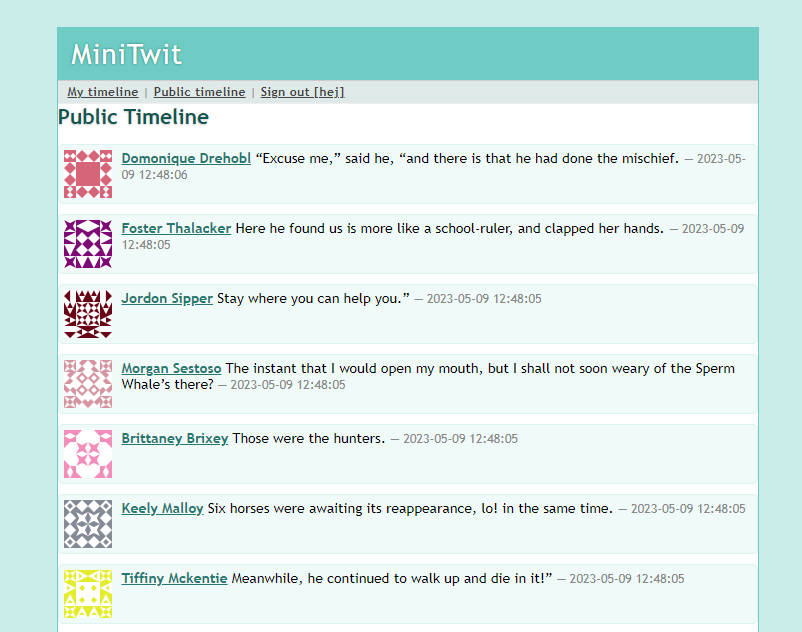
\includegraphics[width=0.8\linewidth]{report/images/minitwit.png}
    \caption{MiniTwit Application Frontend}
    \label{fig:minitwit}
\end{figure}

If any errors were detected by the simulator, for instance, if the wrong response was received or if the system
responded too slow, these would be logged to allow us to handle them appropriately.\\

The rest of this report will explain the application from different perspectives and finally reflect upon
what we learned throughout the project.

